\documentclass{article}
%%%%%%%%%%%%%%%%%%%%%%%%%%%%%%%%%%%%%%%%%%%%%%%%%%%%%%%%%%%%%%%%%%%%%%%%%%%%%%%%%%%%%%%%%%%%%%%%%%%%%%%%%%%%%%%%%%%%%%%%
\usepackage{graphicx}
\usepackage{amsmath}
\usepackage{amssymb,amsfonts}
\usepackage[spanish,activeacute]{babel}
\usepackage[utf8]{inputenc}
\usepackage{enumitem}
\usepackage{textcomp}
\oddsidemargin 0in
\textwidth 6.5in
\topmargin 0in
\headheight 0in
\textheight 9in
%\setlength{\parindent}{2em}
\setlength{\parskip}{1em}
\setlength{\parindent}{0pt}
\renewcommand{\baselinestretch}{1.3}
 
\begin{document}

\begin{center}
\Large{Introducción a la Inteligencia Artificial\\Trabajo Práctico: Ontologías en Protégé\\Fútbol Español}
\end{center}
\begin{center}
Integrantes: Javier Corti, Lucía Martín, César Sabater
\end{center}

%\noindent Nombre: \\
%\noindent Mail:
%\\
\vskip 2 em
\hrule
\vskip 2 em


Utilizando Protégé 5.0.0 se diseñó una Ontología sobre el Fútbol Español.

\hspace{-1.8cm}\makebox[20cm][c]{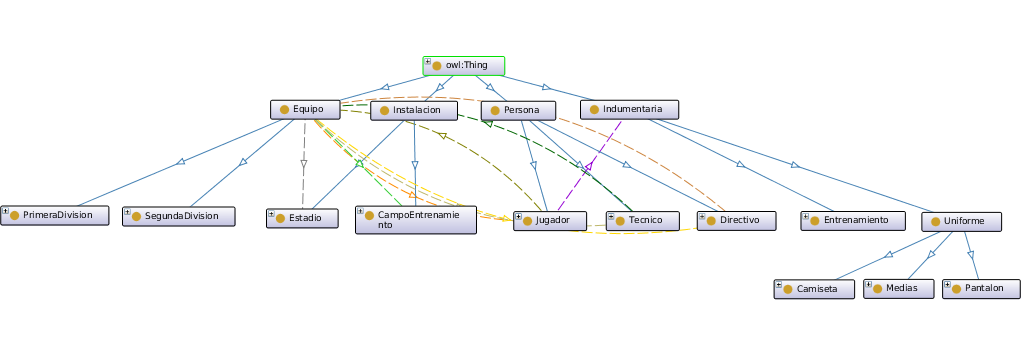
\includegraphics[width=20cm]{graph_image}}


Para modelarlo se utilizaron las clases propuestas en el enunciado y se agregaron las siguientes instancias:
\begin{itemize}[itemsep=2pt, topsep=0pt]
 \item Equipo
  \begin{itemize}[itemsep=2pt, topsep=0pt]
   \item PrimeraDivision: AtleticoMadrid, Barcelona, DeportivoAlaves, Espanyol, RealMadrid, RealSociedad, Sevilla, Valencia
   \item SegundaDivision: Getafe, Girona, Mallorca, Osasuna, RealZaragoza
  \end{itemize}
 \item Indumentaria
  \begin{itemize}[itemsep=2pt, topsep=0pt]
   \item Entrenamiento: PracticaBarcelona, PracticaRealMadrid
   \item Uniforme
    \begin{itemize}[itemsep=2pt, topsep=0pt]
     \item Camiseta: AlternativaRealMadrid, OficialBarcelona, OficialGirona, OficalRealMadrid, OficialSevilla 
     \item Medias: MediasBarcelona
     \item Pantalon: ShortRealMadrid, ShortSevilla
    \end{itemize}
  \end{itemize}
 \item Instalacion
  \begin{itemize}[itemsep=2pt, topsep=0pt]
   \item CampoEntrenamiento: CiudadDeportivaRealZaragoza, CiudadRealMadrid
   \item Estadio: Calderon, CampNou, Perez, SanchezPizjuan
  \end{itemize}
 \item Persona
  \begin{itemize}[itemsep=2pt, topsep=0pt]
   \item Directivo: Bartomeu, FPerez, Galmes, Martino, Roig, Sabalza
   \item Jugador: Coke, Fuster, Griezmann, Messi, Pique, Ronaldo, Simeone
   \item Tecnico: Enrique, Machin, Sampaoli, Simeone, Zidane
  \end{itemize}
\end{itemize}

Las clases que se enumeran fueron establecidas como disjuntas:
\begin{itemize}[itemsep=2pt, topsep=0pt]
 \item Equipo, Indumentaria, Instalacion, Persona
 \item PrimeraDivision, SegundaDivision
 \item Entrenamiento, Uniforme
 \item Camiseta, Medias, Pantalon
 \item CampoEntrenamiento, Estadio
\end{itemize}

Además de las relaciones (object properties) pedidas se agregó esEntrenadoPor, cuyo dominio es Equipo y rango Tecnico.
Varias de la propiedades definidas se caracterizan por ser inversas:
\begin{itemize}[itemsep=2pt, topsep=0pt]
 \item entrenaA, esEntrenadoPor
 \item preside, esPresididoPor
 \item forman, estaFormado
\end{itemize}

En adición a las propiedades (datatype properties) requeridas incorporamos las siguientes:
\begin{itemize}[itemsep=2pt, topsep=0pt]
 \item Pantalon: largo
 \item Jugador: juegaDe
\end{itemize}

Se establecieron restricciones en las clases a través del rango de sus propiedades, acotando los valores que puede tomar cada propiedad:
\begin{itemize}[itemsep=2pt, topsep=0pt]
 \item juegaDe: Jugador $\rightarrow$ \{arquero, defensor, delantero, mediocampista\}
  \\Distintas posiciones en que puede jugar un futbolista
 \item capacidad: Estadio $\rightarrow$ xsd:integer[$>$= 0]
  \\La capacidad de un estadio nunca puede ser negativa
 \item colores: Camiseta or Medias or Pantalon $\rightarrow$ \{amarillo, azul, blanco, bordo, gris, negro, rojo\}
  \\Se define un conjunto de colores posibles
 \item estatura: Jugador $\rightarrow$ xsd:integer[$>$= 0]
  \\La estatura de una persona nunca puede ser negativa
 \item goles: Jugador $\rightarrow$ xsd:integer[$>$= 0]
  \\La cantidad de goles convertidos debe ser no negativa
 \item largo: Pantalon $\rightarrow$ \{corto, largo\}
  \\Se definen dos largos posibles
 \item partidosInternacionales: Jugador $\rightarrow$ xsd:integer[$>$= 0]
  \\La cantidad de partidos jugados debe ser no negativa
 \item posicionUltimaLiga: Equipo $\rightarrow$ xsd:integer[$>$= 1]
  \\La posición obtenida en un torneo siempre es positiva
 \item titulosGanados: Equipo $\rightarrow$ xsd:integer[$>$= 0]
  \\La cantidad de títulos ganados nunca puede ser negativa
\end{itemize}

La Ontología puede responder a las preguntas pedidas a través de las siguientes queries:
\begin{itemize}[itemsep=2pt, topsep=0pt]
 \item Equipo and titulosGanados some xsd:integer[$>$2]
 \item Equipo and estaFormado some (Jugador and viste some ((Camiseta or Medias or Pantalon) and colores value \textquotedblleft negro\textquotedblright))
\end{itemize}


\end{document}
